\section{问题描述}
\subsection{概述}
基于蚂蚁开源的分布式实时图计算引擎TuGraph Analytics提供的⾼阶API编程接口,在LDBC FinBench测试数据集上,完成赛题指定的图模式匹配算法的实现,并尽可能提升算法的整体性能(包含构图、匹配、输出全部过程)。

\subsection{数据简介}
基于TuGraph Analytics的高阶API进行构图操作,将``FinBench数据集''转换为以下图数据格式。

\subsection{数据格式}
具体数据格式信息可参考``LDBC FinBench文档''\cite{ref3} Data Definition 章节.

\begin{figure}[H]
  \begin{center}
    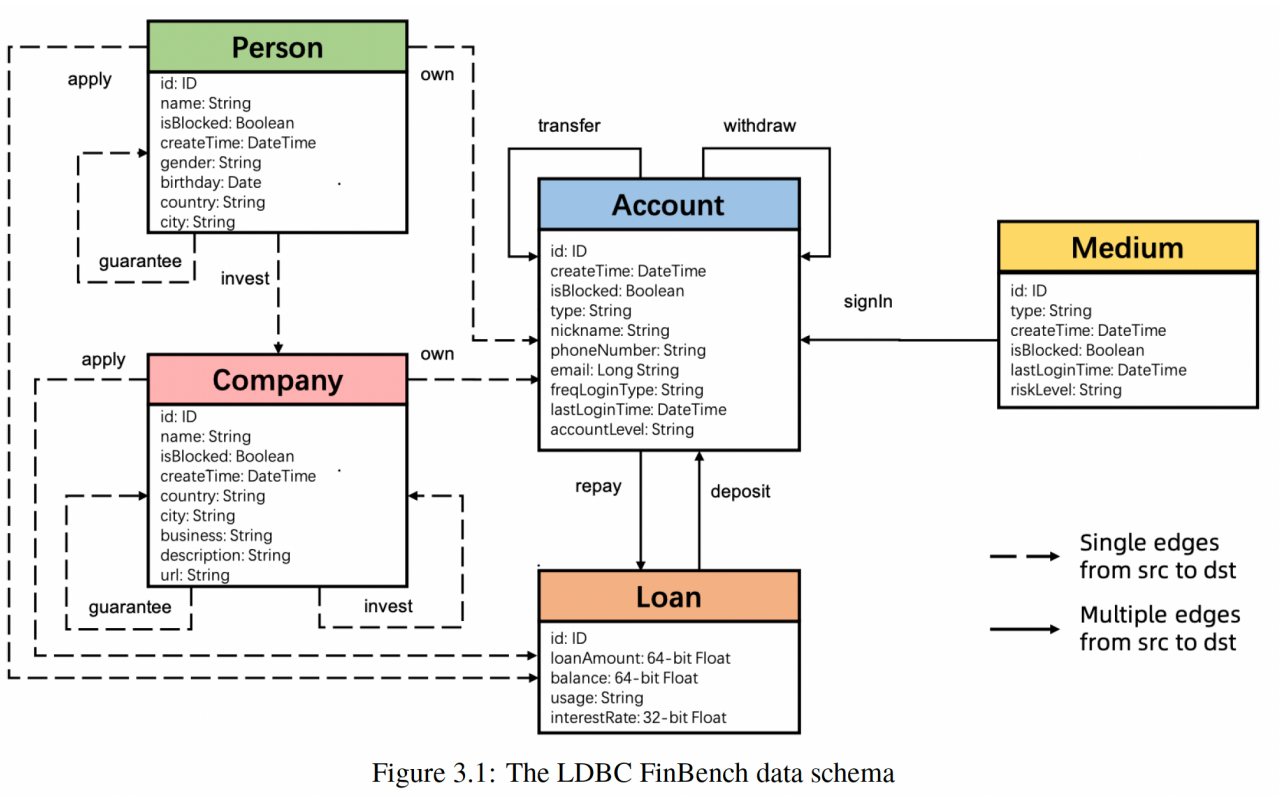
\includegraphics[width=0.95\textwidth]{./figures/蚂蚁2-1-728694.png}
  \end{center}
  \caption{The LDBC FinBench data schema}
\end{figure}

\subsection{数据文件}
\begin{itemize}
  \item 点数据文件:
    \begin{enumerate}
      \item Account.csv
      \item Loan.csv
      \item Person.csv
    \end{enumerate}
  \item 边数据文件:
    \begin{enumerate}
      \item AccountTransferAccount.csv
      \item LoanDepositAccount.csv
      \item PersonApplyLoan.csv
      \item PersonGuaranteePerson.csv
      \item PersonOwnAccount.csv
    \end{enumerate}
\end{itemize}

\subsection{交易闭环搜索问题}
\begin{figure}[H]
  \begin{center}
    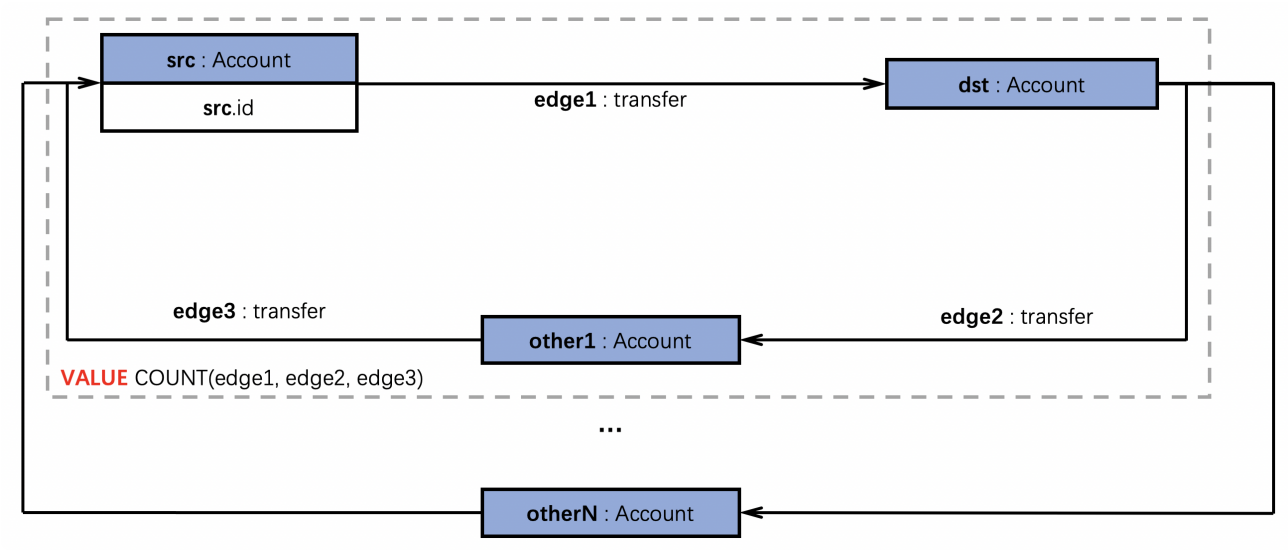
\includegraphics[width=0.95\textwidth]{./figures/蚂蚁改5-264319.png}
  \end{center}
  \caption{交易闭环搜索}
\end{figure}

\begin{itemize}
  \item 目标: 匹配满足以下条件的所有账户src:
    \begin{enumerate}
      \item src 向账户 dst 发起过转账(edge1:transfer)。
      \item dst 向另一个账户 other 发起过转账(edge2:transfer)。
      \item other 向 src 发起过转账(edge3:transfer)。
    \end{enumerate}
  \item 输出
    \begin{enumerate}
      \item id:满足目标条件的 src.id。
      \item value:交易闭环(序列<edge1, edge2, edge3>)中的数量。
    \end{enumerate}
\end{itemize}

\subsection{资金快进快出问题}
\begin{figure}[H]
  \begin{center}
    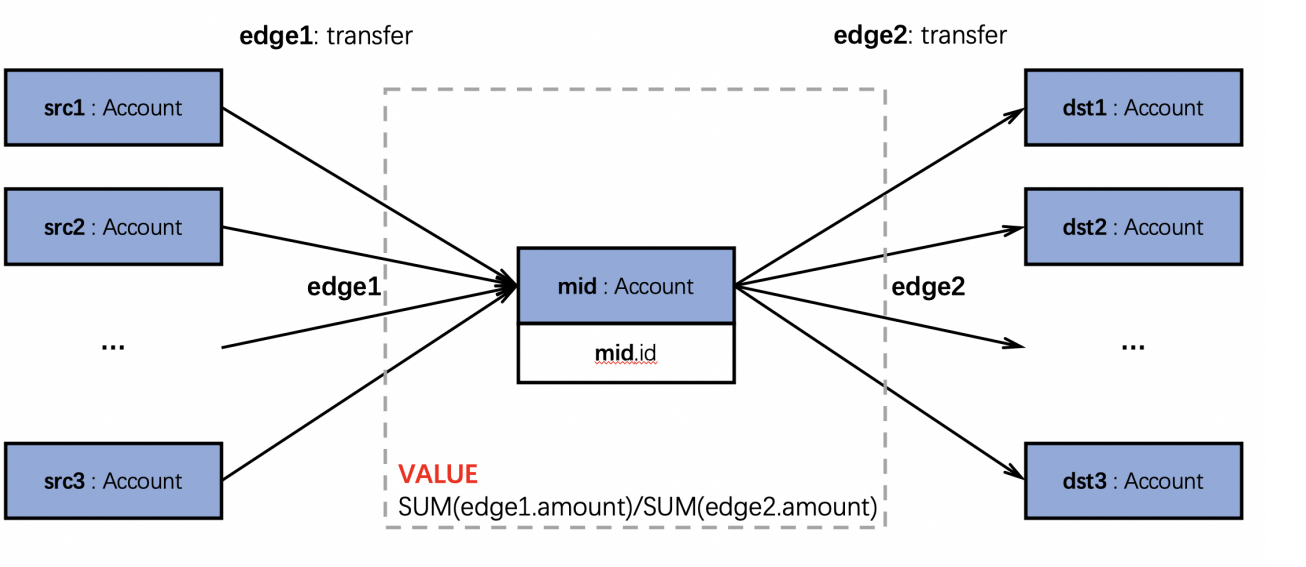
\includegraphics[width=0.95\textwidth]{./figures/蚂蚁改6-546936.png}
  \end{center}
  \caption{资金快进快出}
\end{figure}

\begin{itemize}
  \item 目标: 匹配满足以下条件的所有账户mid:
    \begin{enumerate}
      \item 找到所有向mid发起的转账边(edge1:transfer),至少一条。
      \item 找到所有mid发起的转账边(edge2:transfer),至少一条。
    \end{enumerate}
  \item 输出
    \begin{enumerate}
      \item id:满足目标条件的 mid.id。
      \item value:交易流入流出比,SUM(edge1.amount) / SUM(edge2.amount),小数点后保留2位有效数字。
    \end{enumerate}
\end{itemize}

\subsection{结果格式}
\begin{itemize}
  \item 每个 Case 的结果写到单独的 CSV 文件,文件名为:``result'' + \$\{Case编号\} +
    ``.csv'',如 result1.csv。
  \item 文件内容格式为:
    \begin{enumerate}
      \item 分隔符统一使用:|;
      \item 首行必须是:id|value;
      \item 其中 id 要保证自增顺序(按照数字大小进行排序).
    \end{enumerate}
\end{itemize}

\subsection{测试环境}
\begin{itemize}
  \item CPU: 16vCPU;
  \item 内存: 64 GB;
  \item 硬盘: 满足需求即可.
\end{itemize}
